\chapter{Interpretation of Morphogen Gradients by a Bistable Circuit}
\label{chapter:double-exclusive}
\begin{music}
    \parindent10mm \instrumentnumber{1} \setstaffs1{1} 
    \generalmeter{\meterfrac34} \generalsignature{0}
    \startextract
		\Notes\zq d\qu a \qu f\qu h\enotes\bar
        \Notes\zq h\qu b\hl i\enotes
    \zendextract
\end{music}
\epigraph{\textit{the clear water's surface reflects
growth}}{Serenade of Water --- Ocarina of Time}\section{Preface}

This chapter contains a published article which resulted from an interdisciplinary collaboration in synthetic cell biology with Station B at Microsoft Research Cambridge. The aim of Station B was to improve all phases of the \emph{design--build--test--learn} workflow (Figure \ref{fig:dbtl}). While specific questions in developmental biology were addressed in the publication, the research was conducted with the wider purpose of identifying bottlenecks in synthetic biology workflow and designing software and automation tools to alleviate those bottlenecks. In particular, the workflow should enable the optimisation of experimental conditions that would yield specific design goals within biomanufacturing pipelines. Applications could range from increasing the yield on \emph{leghemoglobin} through the genetic manipulation of synthetic yeast in the production of plant-based meats, to optimisation of transfection protocols for the production of cell-based therapies, through to engineering bacteria or algae for bio-compatible dye production and application.

\subsection{Problem Statement \& Context}

The aim of this project is to reconstitute and control minimal self-organisation mechanisms which are believed play crucial roles in developmental biology. To this
end \textit{E. Coli} has been genetically engineered to produce orthogonal responses to two different input signals --- henceforth this organism will be referred to as the \textit{double exclusive reporter} circuit \cite{Grant2016}. The colony of reporters serve as a reduced model for a multi-cellular organism during embryonic stages of development. While patterns with sharp boundaries have successfully been realised, producing Turing instabilities remains challenging as the system needs to be such that patterns develop before the colony reaches stationary phase. The role of theory and computation in this project is to help identify the
parameter regimes that produce controllable and self-organised patterns.

\subsection{Contributions}

\textbf{Grisha Szep} is co-second author with \textbf{Om Patange} (University of Cambridge, UK). \textbf{Paul Grant}, \textbf{Neil Dalchau}, \textbf{Jacob Halatek} and \textbf{Andrew Phillips} (all Microsoft Research Cambridge, UK) conceived and designed the study. \textbf{Paul Grant} designed and built the genetic circuits. \textbf{Paul Grant}, \textbf{Om Patange} and \textbf{Valerie Coppard} (Microsoft Research Cambridge, UK) performed the experiments. \textbf{Grisha Szep}, \textbf{Jacob Halatek} and \textbf{Neil Dalchau} conceived and implemented theory and modelling and wrote the supplementary information. All authors analysed and interpreted the data. \textbf{Paul Grant} and \textbf{Andrew Philips} wrote the main text. All authors provided input into the manuscript. The contributions of \textbf{Grisha Szep} the main text (Sections \ref{double-exclusive:abstract}--\ref{double-exclusive:cultures}) and supplementary (Appendix \ref{appendix:double-exclusive}) include:
\begin{itemize}
    \item \textbf{Figure 1.b} Spatial simulations of parameterized model
    \item \textbf{Figure 2.a-b} Calculation of region of bistability predicted by the parameterized model using arc-length continuation algorithms
    \item \textbf{Figure 3.b-e} Wrote bespoke inference code for quantification of boundary velocity from microscopy movies and comparison to theoretical model
    \item \textbf{Figure 4.d-e} Spatial simulations of the parametrized model. Novel state-space analysis of boundary formation and bistability
    \item \textbf{Figure S10.c} Spatial simulations analysed in state-space
    \item \textbf{Figure S13} A novel method for quantifying hysteresis in the flow cytometry experiments as population separation
    \item \textbf{Figure S25-S26} Bistability analysis of parametrized models and comparison to qualifications from flow cytometry
    \item \textbf{Figure S27-S33} Simulations of boundary velocity, novel way of understanding them in state space and bespoke inference methods for quantification of boundary velocity from microscopy movies
    \item \textbf{Figure S36} State space geometry for model with feedback loops
    \item \textbf{Supplementary Sections 2.2-2.4} Wrote sections outlining the methods for extracting bistability regions from data and models with and without feedback loops
    \item \textbf{Movies 1-5} Simulations of expression boundary formation
    \item \textbf{Code} Released code with documentation in the GitHub Repository \href{https://github.com/gszep/double-exclusive-reporter}{\texttt{github.com/gszep/double-exclusive-reporter}}
\end{itemize}

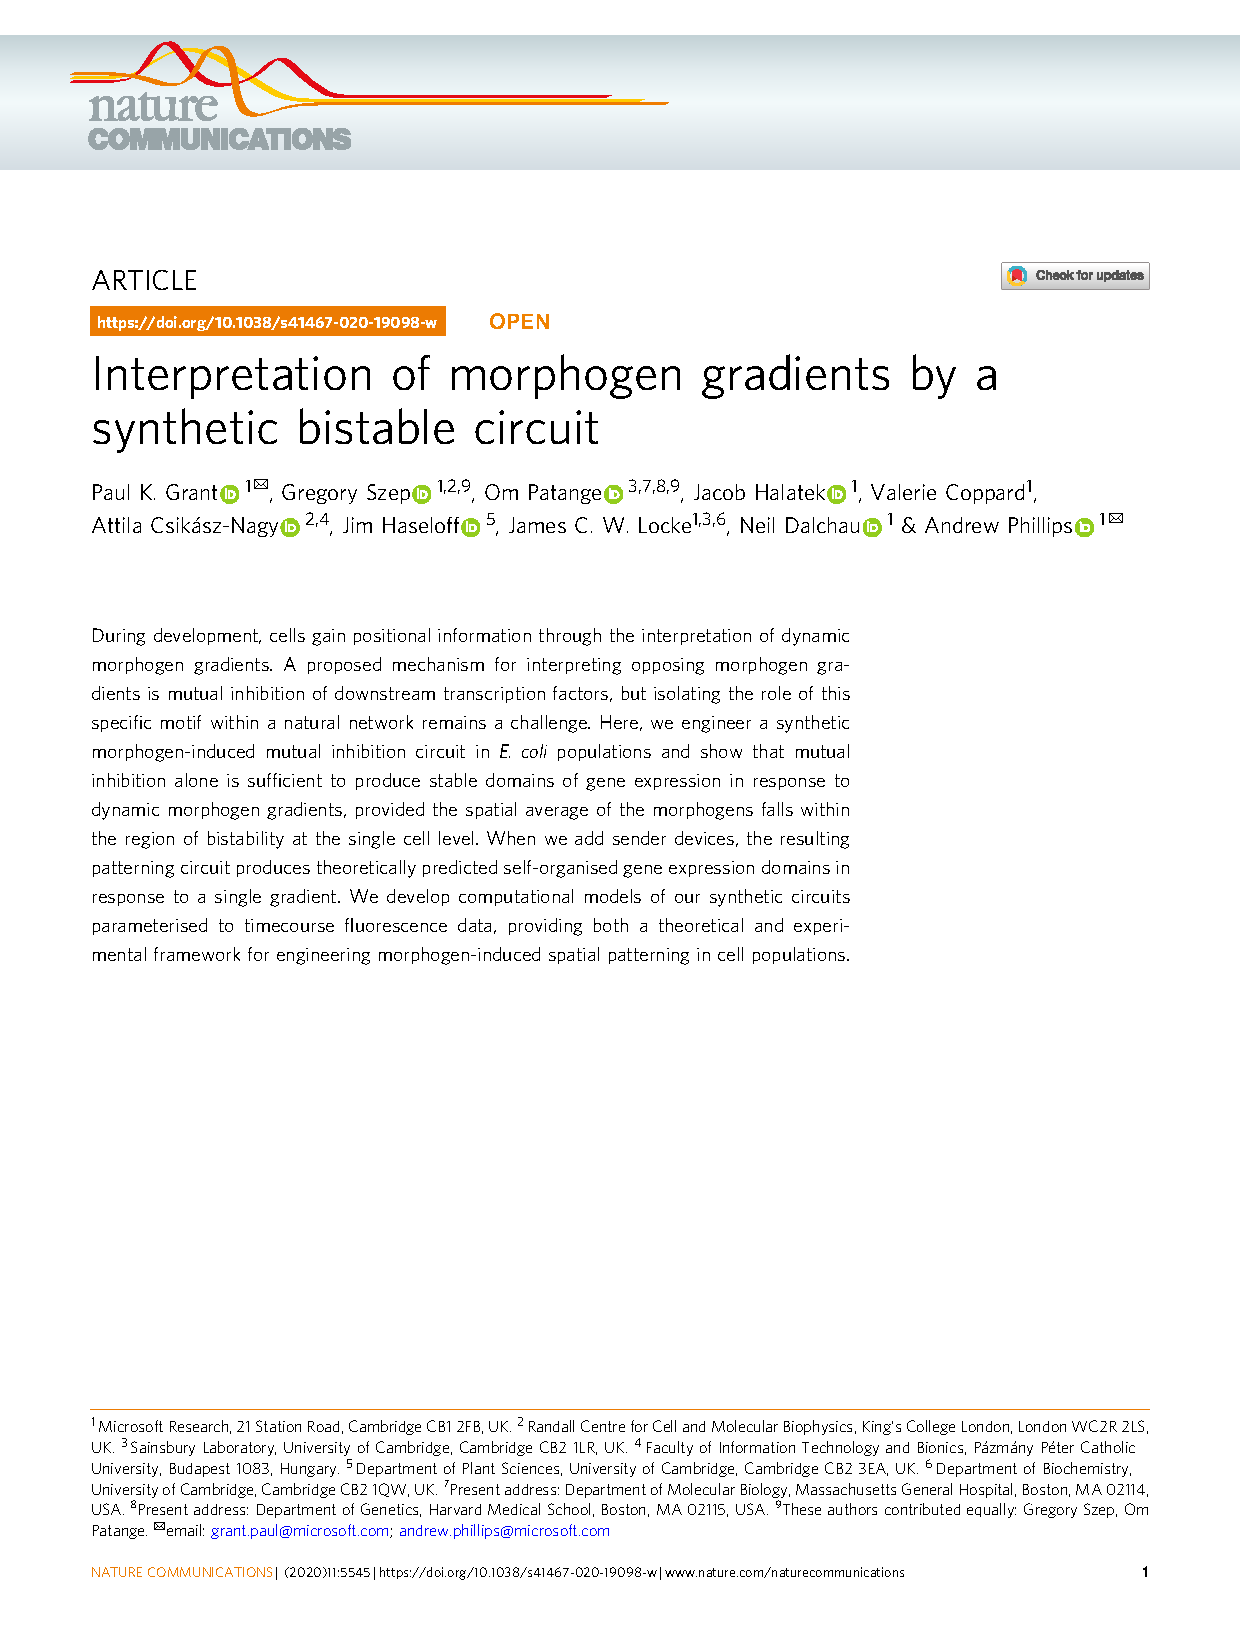
\includepdf[pages=1-8, offset=75 -90, scale=0.85, frame,
        clip,trim=10mm 5mm 10mm 0mm,
        pagecommand={}, addtotoc={
        1,section,1,Abstract,double-exclusive:abstract,
        2,section,1,Introduction,double-exclusive:introduction,
        2,section,1,Results,double-exclusive:results,
        2,subsection,2,Engineering mutual exclusivity,double-exclusive:exclusivity,
        3,subsection,2,Mutual inhibition results in bistability,double-exclusive:bistability,
        4,subsection,2,Hysteresis produces stable boundaries,double-exclusive:boundaries,
        4,subsection,2,A secondary gradient creates self-organised domains,double-exclusive:self-organisation,
        5,section,1,Discussion,double-exclusive:discussion,
        6,section,1,Methods,double-exclusive:methods,
        6,subsection,2,Plasmid construction,double-exclusive:plasmids,
        6,subsection,2,Plate fluorometer assay,double-exclusive:plates,
        6,subsection,2,Flow-cytometric analysis of hysteresis,double-exclusive:flow,
        7,subsection,2,Microfluidics,double-exclusive:microfluidics,
        7,subsection,2,Microfluidics microscopy,double-exclusive:microscopy,
        7,subsection,2,Solid culture assays,double-exclusive:cultures},
    addtolist={
        2, figure, {\textit{Fig. 1}\quad A synthetic gene circuit for morphogen interpretation.}, fig:double-exclusive:overview,
        3, figure, {\textit{Fig. 2}\quad Mutual inhibition produces bistability.}, fig:double-exclusive:bistability,
        5, figure, {\textit{Fig. 3}\quad Formation of stable boundaries.}, fig:double-exclusive:boundaries,
        6, figure, {\textit{Fig. 4}\quad Addition of a Relay circuit creates self-organised domains of gene expression.}, fig:double-exclusive:relay
}]{publications/double-exclusive.pdf}

\section{Afterword}
\label{afterword:inference}

The decision to focus on single cell trajectories and flow cytometry in this study came from the limitations of using microplate data: it is not possible to detect multi-modality in fluorescence distributions from plates that could indicate a population of mixed phenotypes. In order to restore phenotype information, model parameters $\theta$ were estimated using a hierarchical Monte Carlo approach and time-course fluorescence microplate measurements (details of which can be found in Appendix \ref{appendix:double-exclusive:inference}). The time-courses include information about dynamical transients and colony growth in liquid culture. This information was used to estimate parameters that dictate the shape of the steady state manifold. The desired cusp bifurcation, however, lives in state-space rather than the time-domain. Ideally we would estimate parameters for the steady state manifold using the subset of data that tell us about the manifold. This way the parameter search is not restricted by kinetic constraints that are ultimately not part of our design goals. It is not possible to observe the cusp bifurcation in microplate data due to the averaging of signals originating from heterogeneous cell populations. Instead, the cusp bifurcation can be observed in flow cytometry measurements of colonies in exponential phase (Supplementary Figure \ref{fig:double-exclusive:flow-hysteresis}) and microfluidic fluorescence microscopy data (Figure \ref{fig:double-exclusive:bistability}c) where computations on single-cell trajectories reveal the hysteresis loop which must necessarily accompany the cusp. The disconnect between the domain that the data lives in and the domain of the design goals poses the risk of over-fitting the model on undesired information that exists in the data domain.

This motivated investigating \emph{inverse bifurcation analysis} methods that could try and find parameter regimes that lead to desired cusp and limit points directly. However, searching for bifurcating parameter regimes within a model is a difficult task, and few methods exist in the literature. We found some contributions where bespoke methods were applied to specific model structures, but would not generalise to arbitrary models \cite{}. Other approaches were based on sampling parameter sets naively and checking for the existence of a bifurcation \cite{}. But, there was no end-to-end differentiable method that took advantage of bifurcation theory directly. We therefore attempted to fill this gap in the literature by developing a methodology based on differentiable continuation in Chapter \ref{chapter:inference}. In doing so, we have elucidated the importance of fitting qualitative before quantitative features within datasets.